\documentclass[conference]{IEEEtran}
\IEEEoverridecommandlockouts

\usepackage{color} %red, green, blue, yellow, cyan, magenta, black, white
\definecolor{mygreen}{RGB}{28,172,0} % color values Red, Green, Blue
\definecolor{mylilas}{RGB}{170,55,241}

% The preceding line is only needed to identify funding in the first footnote. If that is unneeded, please comment it out.
\usepackage{cite}
\usepackage{amsmath,amssymb,amsfonts}
\usepackage{algorithmic}
\usepackage{graphicx}
\usepackage{textcomp}
\usepackage{appendix}
\usepackage{xcolor}
\usepackage{listings}
\usepackage{fancyhdr}
\usepackage{float}
\def\BibTeX{{\rm B\kern-.05em{\sc i\kern-.025em b}\kern-.08em
    T\kern-.1667em\lower.7ex\hbox{E}\kern-.125emX}}
\begin{document}

\thispagestyle{fancy}
\cfoot{}
\renewcommand{\headrulewidth}{0pt}
\renewcommand{\footrulewidth}{0pt}
\pagestyle{fancy}
\rfoot{\thepage}
\title{SSY 135 Project part 1}


\author{\IEEEauthorblockN{Group E:}

\and
\IEEEauthorblockN{Oskar Claeson}
\and
\IEEEauthorblockN{Erik Tilly}
\and
\IEEEauthorblockN{Yuling Zhang}
\and
\IEEEauthorblockN{Haitham Babbili}
}

\maketitle

\section{Introduction}
The objective of this paper is to provide a small basis for understanding both Rayleigh and Rician flat fading channels. This is done through simulations using two main methods, which are known as the Filter method and the Spectrum method. This paper explains how to use the methods in order to simulate a Rayleigh and Rician fading channel with a Jake's Doppler spectrum. In order to assess the channels, results from different tools are analyzed. These tools are the Power Spectral Density (PSD), Probability Density Function (PDF), Cumulative Distribution Function (CDF) and the Auto-Correlation Function (ACF). Also, the different advantages and/or disadvantages of using either method is discussed, to provide a better understanding of the wireless channels.

\section{Rayleigh and Rician Flat Fading channels}
This section is the documentation of how the channels were created. The base method describes the implementation of a Rayleigh channel while it then is changed according to the equation \ref{rician} to create a Rician channel for $K_{c}$ larger than $0$. Comparing Rayleigh and Rician channel, Rician has a line of sight(LOS) component whereas Rayleigh does not.  The K-factor is used to describe a Rician fading channel which is defined as the ratio of signal power in the dominant component  over the other multipath components . Thus, the K-factor is found as:  $K = \frac{s^2}{2\sigma ^2}$ \\In this project the power of the LOS component is represented by $k_{c}$. When the Rician channels are generated, it's made sure that they are normalized in order for the channel to be of unit energy $ \mathbb{E}(|c(nT_{s})|^2) = 1$. For $k_{c} = 0,1,10$, he $K$ factor is thus $0, 0.5, 50$. The $K$ factor is proportional to the value of $k_c$. Based on \ref{rician}, when $k_{c} = 0$, it is exact Rayleigh channel and, actually, Rayleigh is part of the Rician channel. 

    \begin{align}
        c_{Rician}(nT_{s}) = c_{Rayleigh}(nTs) + k_{c} 
        \label{rician}
    \end{align}

The channels are implemented with a "filter method" and a "spectrum method" after the parameters are determined and checked that they full fill the requirements. 

\subsection{Determine the parameters}
    The Doppler frequency is calculated as: $$ f_{D} = \frac{v\times f_{c}}{c} \thickapprox 55.3333 [Hz]$$
    To avoid aliasing, the value of $T_s$ should satisfy: $1/T_{s} > 2f_{D}$. Thus the maximum tolerated $T_s$ to avoid aliasing is $T_{s} < 0.009 [s] = 9 [ms]$. The provided $T_{s} = 0.1 ms$ is lower than the maximum $9 ms$. Therefore, $T_{s} = 0.1 ms$ meets this requirement and can be used as sample time.
    
 
    When estimating the PSD, the quality depends partly on the window size. The shorter the window size is, the poorer result and larger variation. While the window size is increased, better performance is obtained, but at the same time if the size exceed the frequency resolution some noise will occur. This resolution can be calculated accordingly: 
    $$f_{res}  = \frac{f_{s}}{N_{s}} = \frac{1}{T_{s}N_{s}}$$ $$f_{res}  = \left<0.8-1\right>$$
    
A factor was calculated according to Parseval's theorem in equation \ref{parseval}. 
\begin{equation*}
    E = \int_{-\infty}^{+\infty} |x(t)|^2 dt = \frac{1}{2\pi}\int_{-\infty}^{+\infty}|X(\omega)|^2 dw
    \label{parseval}
\end{equation*}


\subsection{Filter method}
To generate the channel using the Filter method, first choose $T_s$ such that no aliasing can occur. Secondly, choose number of samples $N_s$ and make sure this window size gives a good resolution. The filter vector $g(nT_{s})$ is generated in the following way, where  $n = -NT_s,...,NT_s$ and N is a chosen length:
\begin{equation}
   g(t)  = \mathcal{F}^{-1}[\sqrt{S_{c}(f)}] =
\begin{cases}
    \frac{\mathcal{J}_{1/4}(2\pi f_{D}\mid t \mid)}{\sqrt[4]{\mid t \mid}},\quad t\neq0\\
    \frac{\sqrt[4]{\pi f_{D}}}{\Gamma(5/4)},\quad t = 0
\end{cases}
\end{equation}
Where $\mathcal{J}$ is the Bessel function, $\Gamma$ is the gamma function. The vector length should be carefully chosen as a small N leads to artifacts in the PSD and a large N will lead to a high complexity. The filter vector $g$ should be normalized to make sure it has the unit energy.  In order to simulate the channel this filter vector $g$ is convolved with independent samples $x(nT_{s})$ from a complex Gaussian distribution of length $N_{s}$ which are randomly generated as: 
\begin{equation}
    x = (randn(N_s,1) + j\cdot randn(N_s,1))\cdot a
    \label{randn}
\end{equation}
where $a$ is a constant to ensure that the samples of $x$ has unit-variance. The resulting channel $c$ has length $N_s+2N$ due to transients following the convolution operation, which should be discarded.

\subsection{Spectrum method}

Provided that the used parameters fulfill the requirements stated in the previous section, the spectrum method makes use of the Doppler spectrum in the frequency domain, which is the Fourier transform of the ACF. Since the Doppler spectrum is band limited to [$-f_D, f_D$] its only non zero between those frequencies and zero otherwise which is shown in \ref{specdoplerdpread}. In this project samples for only the positive side were generated and then flipped to create the negative half of the spectrum since these should be the same. 

\begin{equation}
\begin{split}
S_c(f) =  \begin{cases} \frac{1}{\pi f_D}\frac{1}{\sqrt{1-(f/f_D)^2}} \quad \mid f\mid \leq f_D \\
0 \quad\quad{otherwise}
\end{cases}
\end{split}
\label{specdoplerdpread}
\end{equation}

When the Doppler spectrum is constructed according to \ref{specdoplerdpread}, with $f_{s}$ as the upper limit, $G(f)$ is found by taking the square root of $S_c$. $G_{p}(f) $ is the periodic version of $G(f)$ and to create $G_{p}(f) $ the $G(f)$ is padded with zeros between the two halves such that the total length is $N_s$. The next step in the process is to generate samples from a complex Gaussian distribution denoted $X$ created as in \eqref{randn} with the same length as $G_p(f)$, i.e $N_s$. Then $G_p(f)$ is multiplied with $X$ to create a vector $C$ ,which in time domain corresponds to a convolution. In order to get the channel response $c(nT_s)$ and the vector $C$ is inverse discrete Fourier transformed. To make sure that the channel $c$ has unit variance a scale factor $a$ is calculated using Parseval's theorem which is multiplied with the samples $X$ before the multiplication. 
     
\section{Simulations of different Rician channels}
In this section the simulations is presented and analysed. The different simulations that are performed as PSD, CDF, PDF and ACF. The PDF, CDF and ACF are performed with different $k_{c}$ values.     

\subsection{Power Spectral Density simulation}
    In figure \ref{PSD}, the estimated PSD of the simulated channels are plotted vs the theoretical PSD. The plot show that both methods have slightly more power compared to the theoretical PSD for frequencies lower than the Doppler frequency, however in general, the form of the curves are matching. And for both of the methods, there are larger variance appearing. This is expected since the theoretical curve is calculated without any noise. When studying how the curves are behaving above the Doppler frequency the filter method and spectrum method differ with about $10 dB$, whereas the theoretical is zero-valued. This indicates that the spectrum method is better at suppressing the higher frequencies since it has a steeper angle when cutting of the higher frequencies.
    
    \begin{figure}[H]
        \centering
        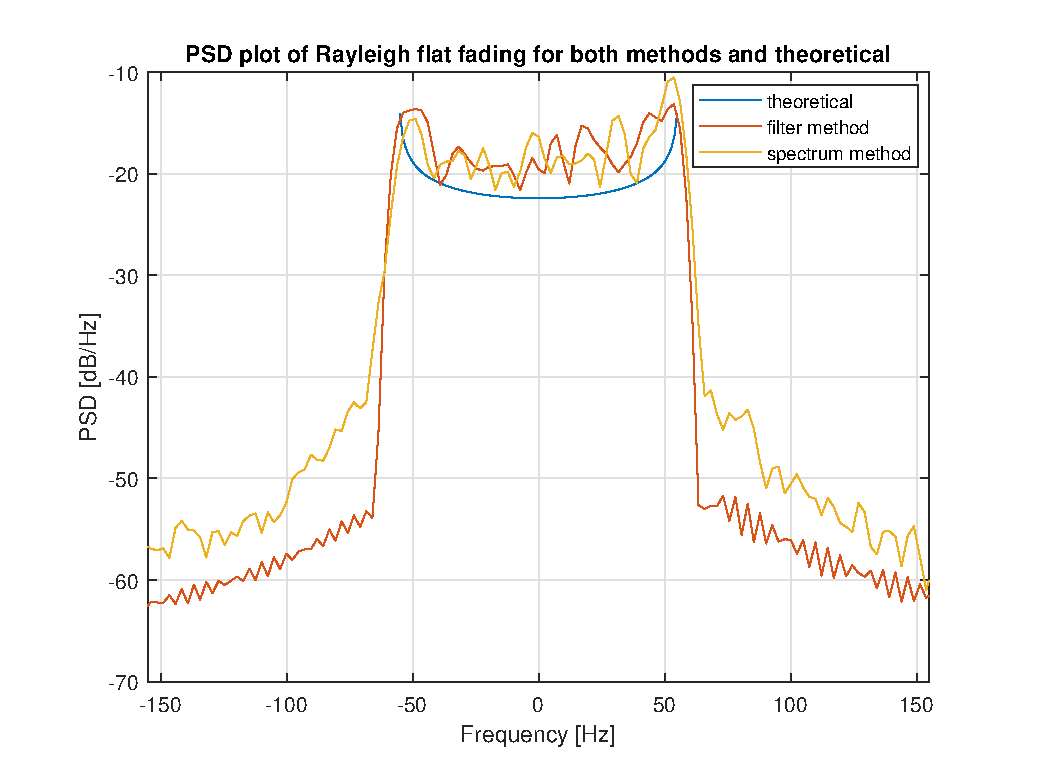
\includegraphics[width = \linewidth]{Figures/PSD_test.eps}
        \caption{Estimate PSD compared with theoretical}
        \label{PSD}
    \end{figure}

\subsection{Probability Density Function }
    In this section, a comparison between the theoretical PDF with the estimated Rician PDF is made with 3 different values of $k_{c}$. These comparisons are plotted in figure \ref{pdf}.
    
    When $k_{c}$ = 0, it can be seen that the PDF is centered around 1.25, which is expected since that is how a Rayleigh distribution looks like.
    If $k_{c}$ is increased to 1, a LOS component is present. This however, does not generate a significant change compared to the $k_{c}$ = 0 channel since according to the K factor, a $k_c$ = 1 gives that the ratio of the LOS component compared to the rest is 0.5 and thus slightly changes the shape.  
    For the larger values of $k_{c}$, in this project, is chosen as 10, the LOS component is much more dominant over the non-LOS components which leads to that the Rician PDF resemble a Gaussian distribution centered around the value of the LOS component, in this case 10. 
    For all values of $k_c$, both simulated methods seem to provide a more narrow curve compared to the theoretical curve which could be due to that these methods normalize the channels to get a unit-variance.
  
    \begin{figure}[H]
        \centering
        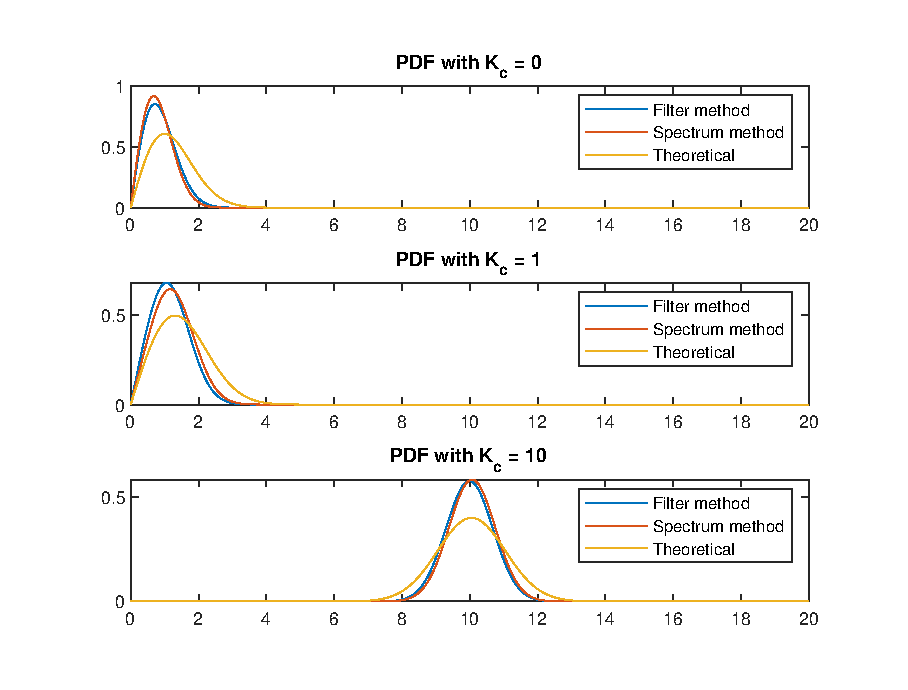
\includegraphics[width = \linewidth]{Figures/PDF_test2.eps}
        \caption{Comparison of the estimated PDFs of the filter and the spectrum method compared to the theoretical channel with different $k_{c}$.}
        \label{pdf}
    \end{figure}
    
\subsection{Cumulative Distribution Function}  
    %The CDF at $k_{c}$ = 0 has normal distribution since it is the Rayleigh fading. As we increase $k_{c}$ to one, there is no such different since non-LOS is still the dominant. Hence, when $k_{c}$ = 10, the mean value shifts to 10.
    
    The CDF of the simulated channels and the theoretical are shown in figure \ref{cdf}.The CDF of the Rayleigh distribution i.e $k_{c}$ = 0 can be seen as the Rician CDF with K = 0. The plot clearly show that the value of $k_c$ (or the LOS component) has an impact on the CDF. As $k_{c}$ is increased, the distribution shifts further to the positive direction on the x-axis which can be seen as an implication of higher SNR. For the increase of $k_c$ from 0 to 1 the change is very slight. However, when $k_{c}$ is increased to 10, the dependency on the K-factor is more obvious as this shifts the curve to be centered at 10.
    
  \begin{figure}[H]
        \centering
        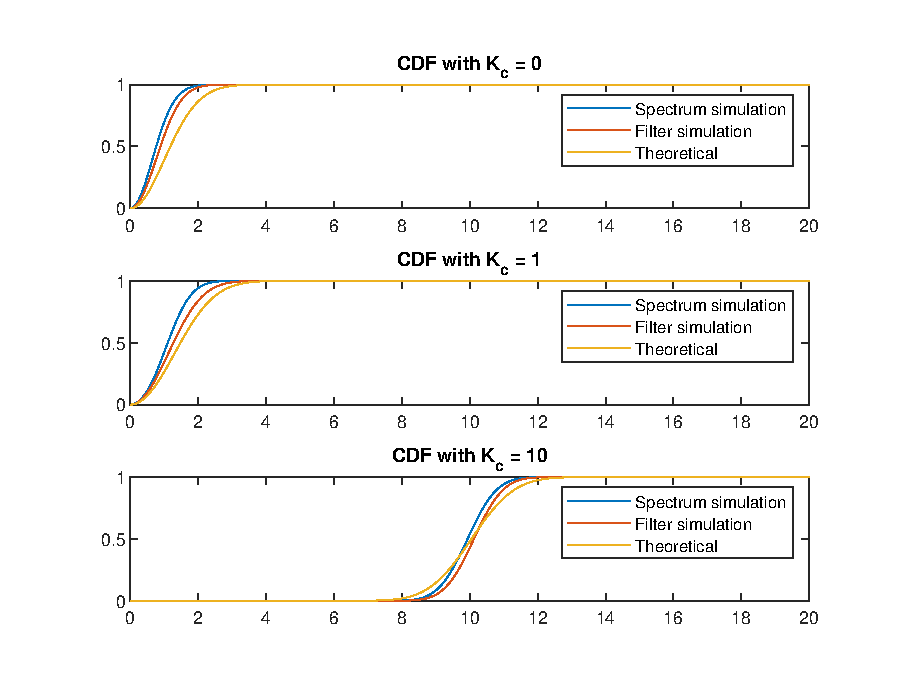
\includegraphics[width = \linewidth]{Figures/CDF.eps}
        \caption{Comparison of the estimated CDFs of the filter and the spectrum method compared to the theoretical channel with different $k_{c}$.}
        \label{cdf}
    \end{figure}
    
\subsection{Auto-Correlation Function}
    
    
    The auto-correlation functions of both simulations and the theoretical is shown in figure\ref{acf}, where the theoretical ACF is given by the following equation:
    \begin{equation}
    A_c({\Delta}t) = J_0(2{\pi}f_D{\Delta}t) + k_c^2
    \label{eqn:acf}
    \end{equation}
    From inspecting the plot it seems as if the shape of the ACF for both methods are more similar to the theoretical one for higher values of $k_c$ but with a small error in amplitude as it seems like there is more correlation than expected when compared to theoretical values. The amplitude of the ACF is heavily dependant on the $k_c$ value as the ACF contain a factor $k_c^2$. As can be seen in the plots, the correlation peaks or increases once again on points other than at zero, which could be a case of periodicity in both methods.
    \begin{figure}[H]
        \centering
        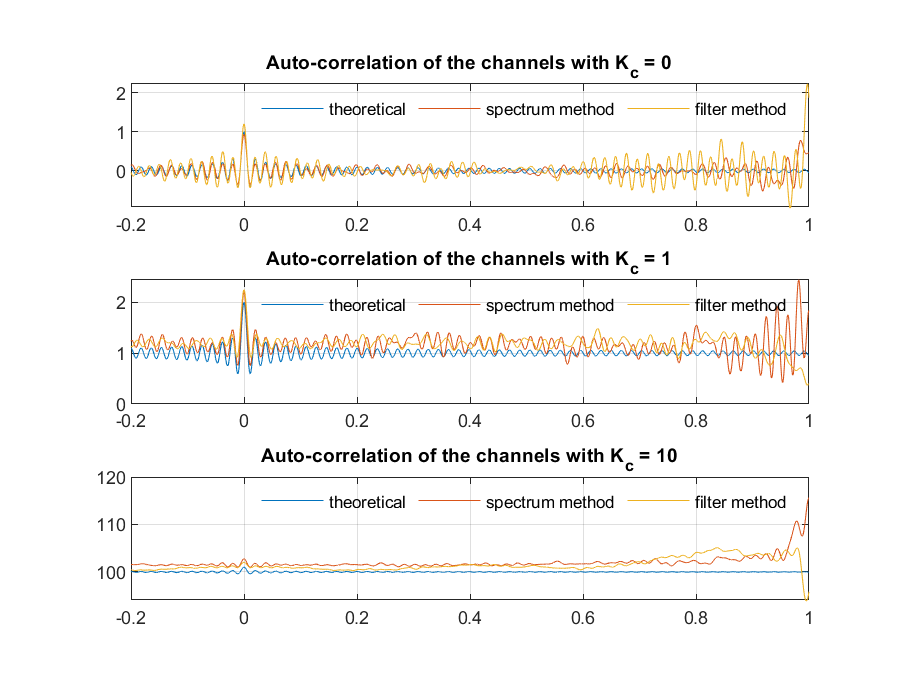
\includegraphics[width = \linewidth]{Figures/ACF.eps}
        \caption{Comparison of the estimated ACFs of the filter and the spectrum method compared to the theoretical channel with different $k_{c}$.}
        \label{acf}
    \end{figure}
    
\subsection{Discussion part 1}

    One advantage of using the spectrum method over the filter method is that it is less complex to perform a simple multiplication compared to the complex convolution operation used in the filter method. This makes the spectrum method quicker. Another advantage of using the spectrum method is that it is more efficient to remove unwanted frequencies, which was shown in the PSD analysis. A disadvantage of choosing the spectrum method over the filter method is that when the window size, i.e $N_s$ is very large it takes up a lot of memory or computer capacity which leads to the decision that for very large $N_s$ the filter method is the only viable choice albeit a much slower one.
    
\section{Time and Frequency-Varying Rician Fading Channels}
\label{task2}
In this task there are 18 figures plotted of different combinations of $f_dT_s$, number of taps $L$ and values of $K_c$ all with $N = 300$ time samples and $M = 64$ frequency samples. These figures are shown in appendix A.
    The delay spread can be calculated as: $$LT_{s} \geq \tau_{DS} \Rightarrow \tau_{DS} = 
    \begin{cases}
        0.1ms,& \text{L=1} \\
        0.2ms,& \text{L=2} \\
        0.3ms,& \text{L=3}
    \end{cases}$$
    To calculate the velocity, the following formula is used:
    $$v = \frac{f_{D}T_{s}\cdot c}{f_{c}\cdot T_{s}}$$
    which gives that
    $$ v = 
    \begin{cases}
       150m/s=540km/h,& \text{$f_{D}T_{s}=0.1$}\\
       7.5m/s=27km/h,& \text{$f_{D}T_{s}=0.005$}
    \end{cases}$$
    
    % fdTs
    The value of $f_{d}T_{s}$ corresponds to the user velocity. From figure \ref{01_10_3} and \ref{0005_10_3}, it is apparently to see that the figure, which has lower value of $f_{d}T_{s}$ is much smoother than the other channels with the same $k_{c}$ and $L$. This is due to lower user velocity and more stable channels since the coherence time is longer for slower movements.
    
    % kc
    With fixed values of $f_{d}T_{s}$ and $L$, and only increasing values of $k_{c}$ the power of the LOS component increase. With $k_{c}$ = 0 the channel is a Rayleigh channel and with higher $k_{c}$ the channels show clearer plots due to less interference from multipath channels.  This can be seen by evaluating figures \ref{0005_1_2} \& \ref{0005_10_2}.
    
    % L
    $L$ means the number of taps. The higher value of $L$, the faster varying will occur along the frequency domain, shown in figure \ref{01_0_1}, \ref{01_0_2} and \ref{01_0_3}. Therefore, when $L = 1$ and do the Discreate Fourier Transform(DFT) of the channel response $C$, it shows as constant amplitude with varying frequency. With increasing value of $L$, more paths are added, which in turn makes the channel response vary in more than one directions. After DFT, there are different values of amplitude corresponds to different frequency value.

    
  
\section{Members contribution}
The way this project was done to first have all members on their own try to figure out the MATLAB simulation part and then together discuss the solutions. Due to different levels of experience in MATLAB, the simulations were mainly done by Yuling and Oskar, where Erik helped with troubleshooting and small fixes. Haitham tried as best he could and was present in discussions of how the implementations were made and gave inputs. Everybody does effort to write report. The bulk of the texts about theory and methods were written by Yuling, Haitham and Erik, whereas Oskar fixed figures, structure, language and sections such like this one, Erik also helped with structure.

\newpage
 
\newpage
\begin{appendices}
\section{}

    The 18 combinations of $L$, $f_{D}T_{s}$ and $k_{c}$ magnitude time and frequency-varying channel responses from Section \ref{task2} are plotted here.

    \begin{figure}[H]
        \centering
        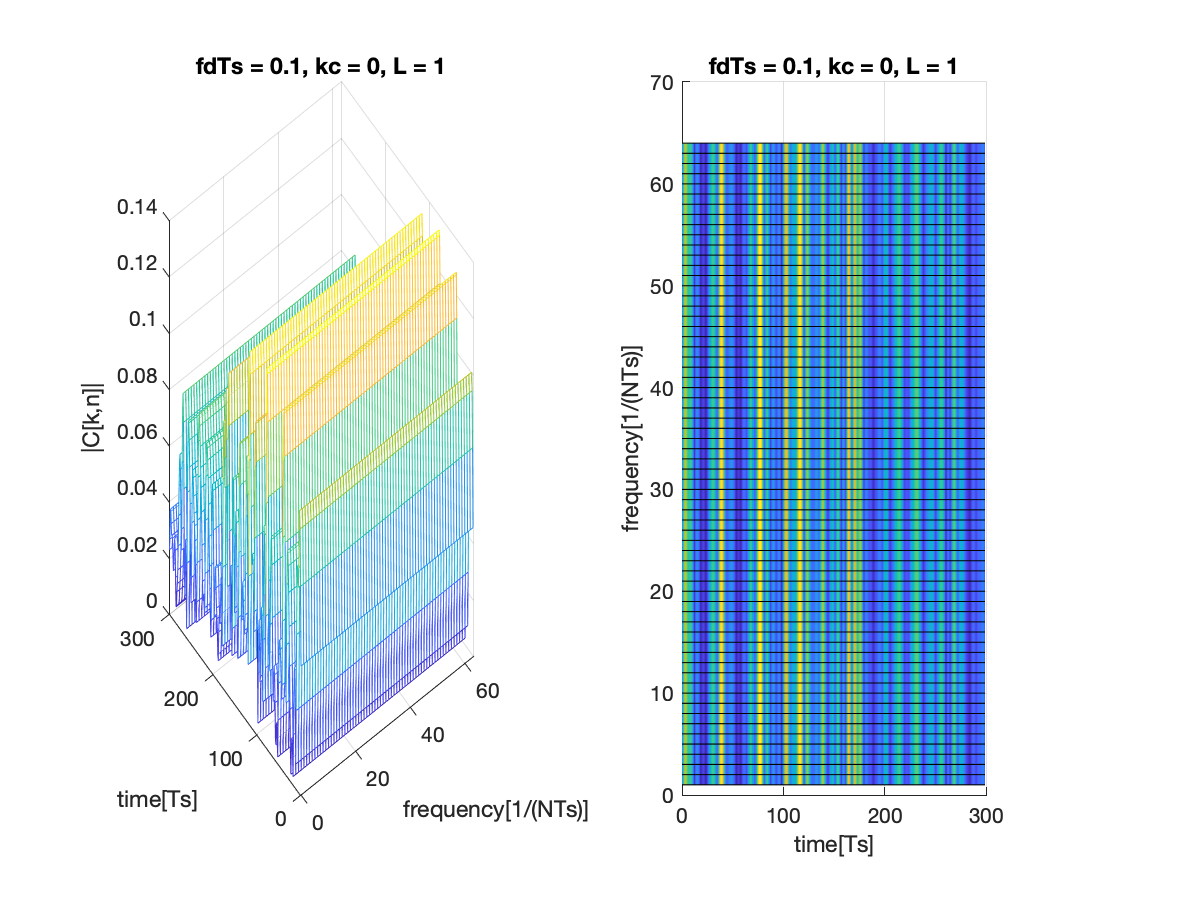
\includegraphics[width = \linewidth]{Task2/01_0_1.eps}
        \caption{$f_{D}T_{s}=0.1$,$k_{c}=0$,$L=1$}
        \label{01_0_1}
    \end{figure}
    \begin{figure}[H]
        \centering
        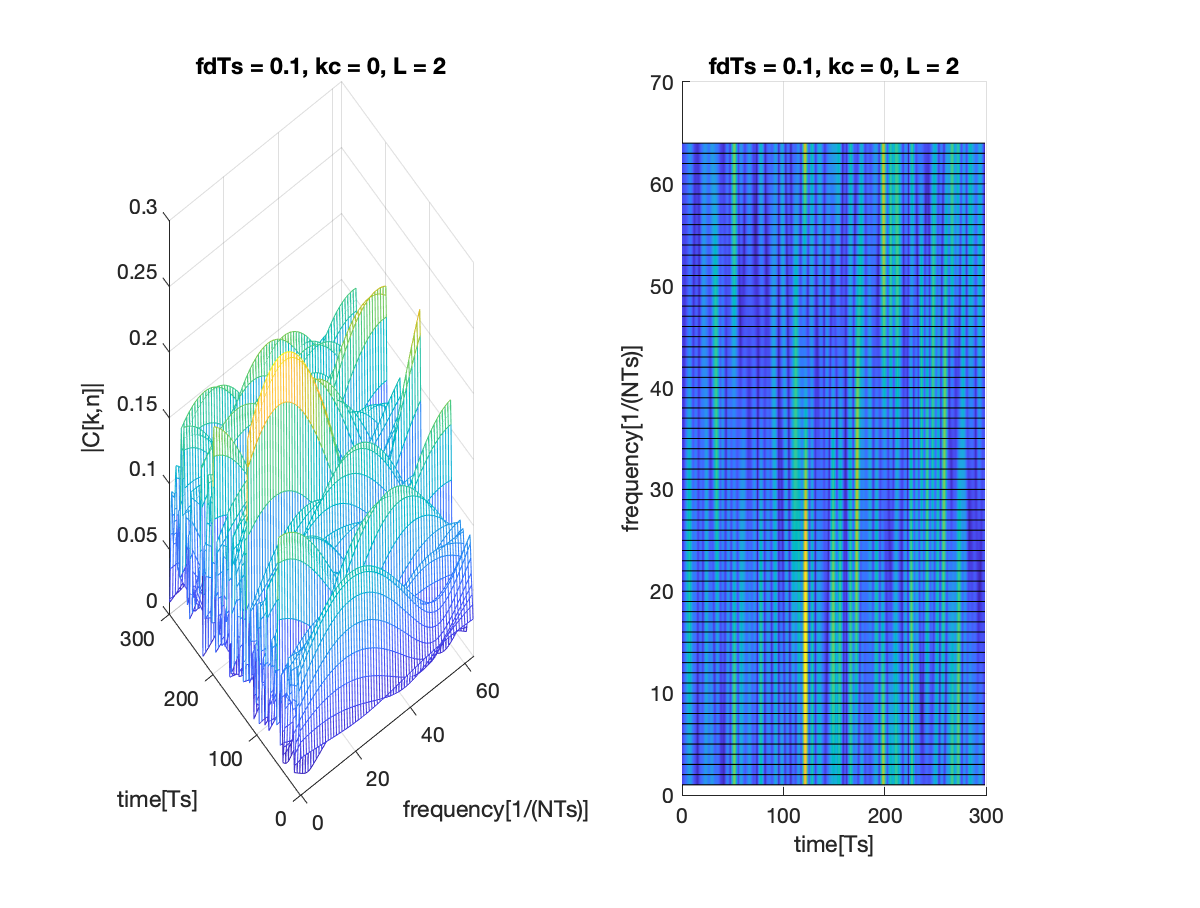
\includegraphics[width=\linewidth]{Task2/01_0_2.eps}
        \caption{$f_{D}T_{s}=0.1$,$k_{c}=0$,$L=2$}
        \label{01_0_2}
    \end{figure}
    \begin{figure}[H]
        \centering
        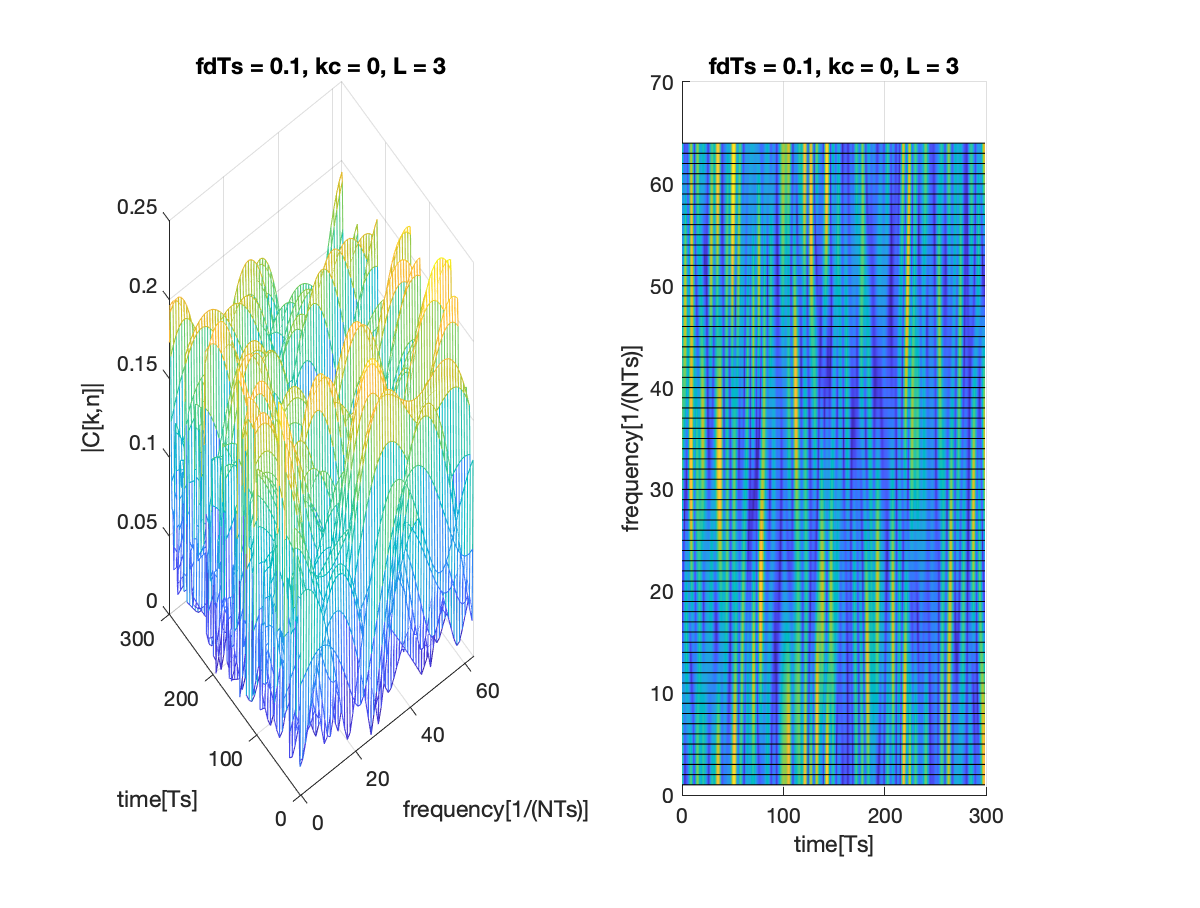
\includegraphics[width=\linewidth]{Task2/01_0_3.eps}
        \caption{$f_{D}T_{s}=0.1$,$k_{c}=0$,$L=3$}
        \label{01_0_3}
    \end{figure}
    \begin{figure}[H]
        \centering
        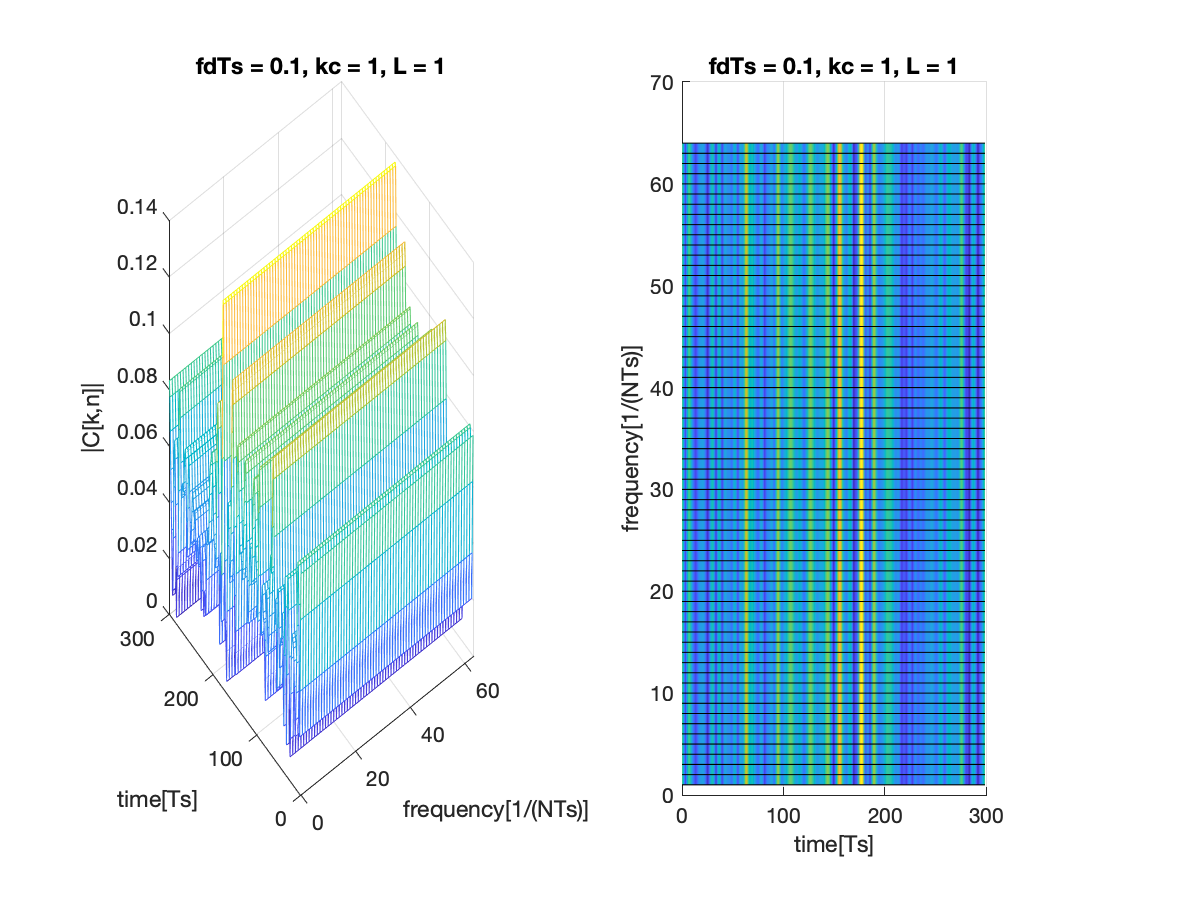
\includegraphics[width=\linewidth]{Task2/01_1_1.eps}
        \caption{$f_{D}T_{s}=0.1$,$k_{c}=1$,$L=1$}
        \label{01_1_1}
    \end{figure}
    \begin{figure}[H]
        \centering
        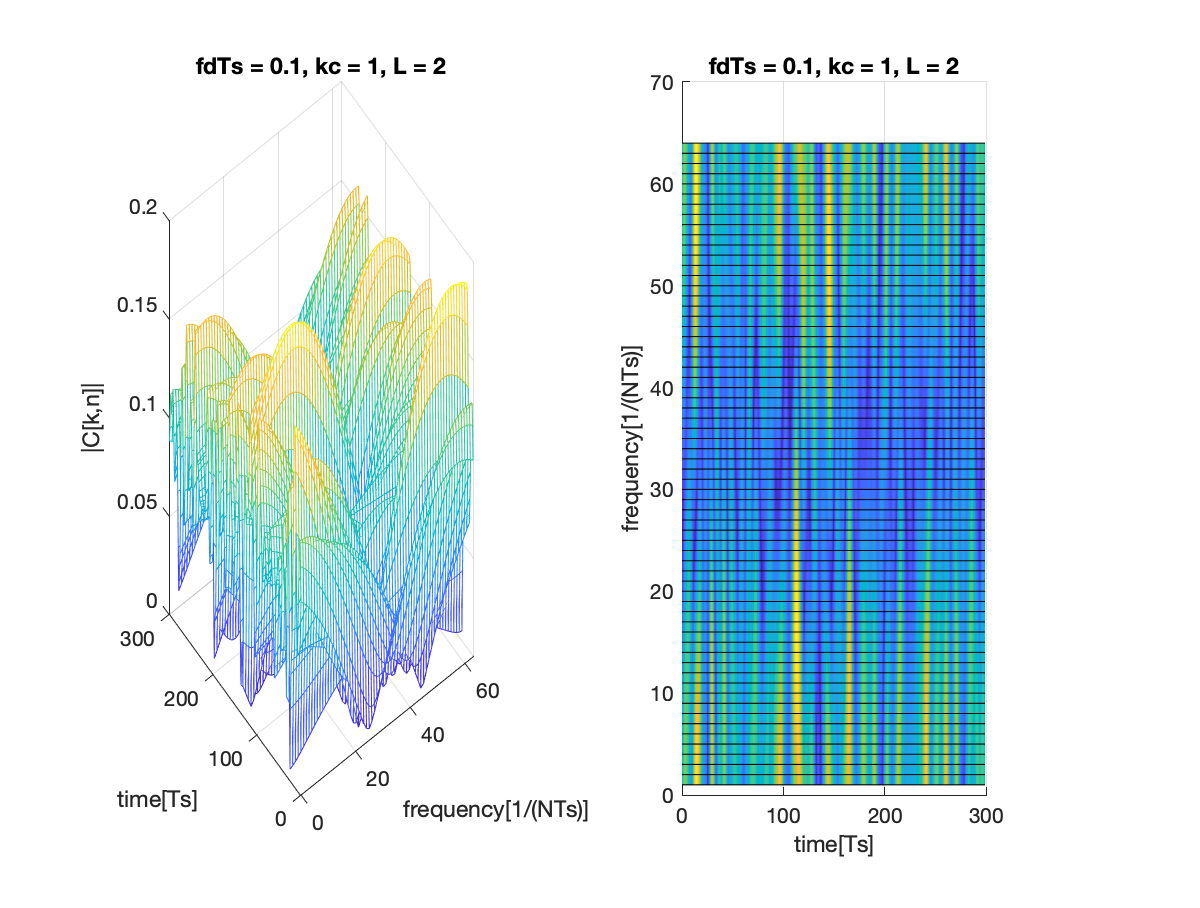
\includegraphics[width=\linewidth]{Task2/01_1_2.eps}
        \caption{$f_{D}T_{s}=0.1$,$k_{c}=1$,$L=2$}
        \label{01_1_2}
    \end{figure}
    \begin{figure}[H]
        \centering
        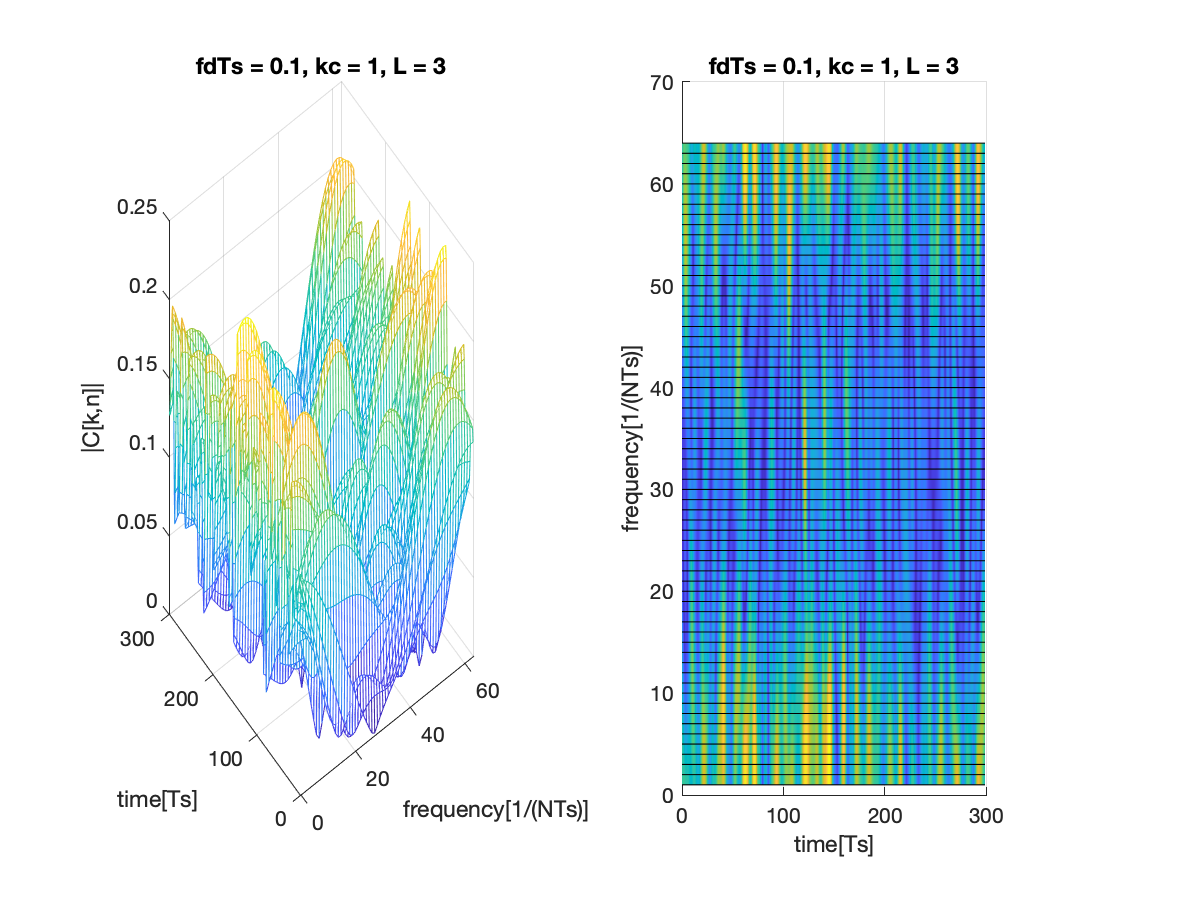
\includegraphics[width=\linewidth]{Task2/01_1_3.eps}
        \caption{$f_{D}T_{s}=0.1$,$k_{c}=1$,$L=3$}
        \label{01_1_3}
    \end{figure}
    \begin{figure}[H]
        \centering
        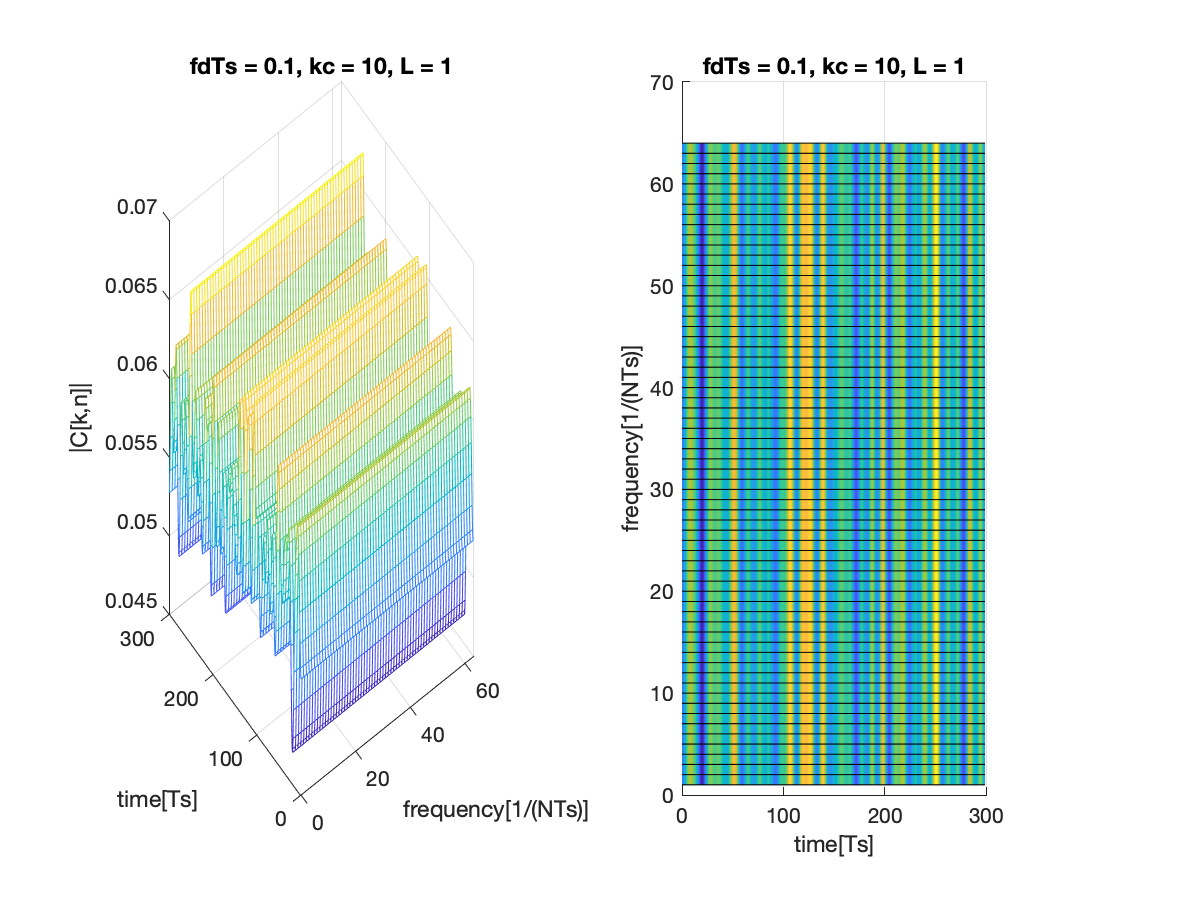
\includegraphics[width=\linewidth]{Task2/01_10_1.eps}
        \caption{$f_{D}T_{s}=0.1$,$k_{c}=10$,$L=1$}
        \label{01_10_1}
    \end{figure}
    \begin{figure}[H]
        \centering
        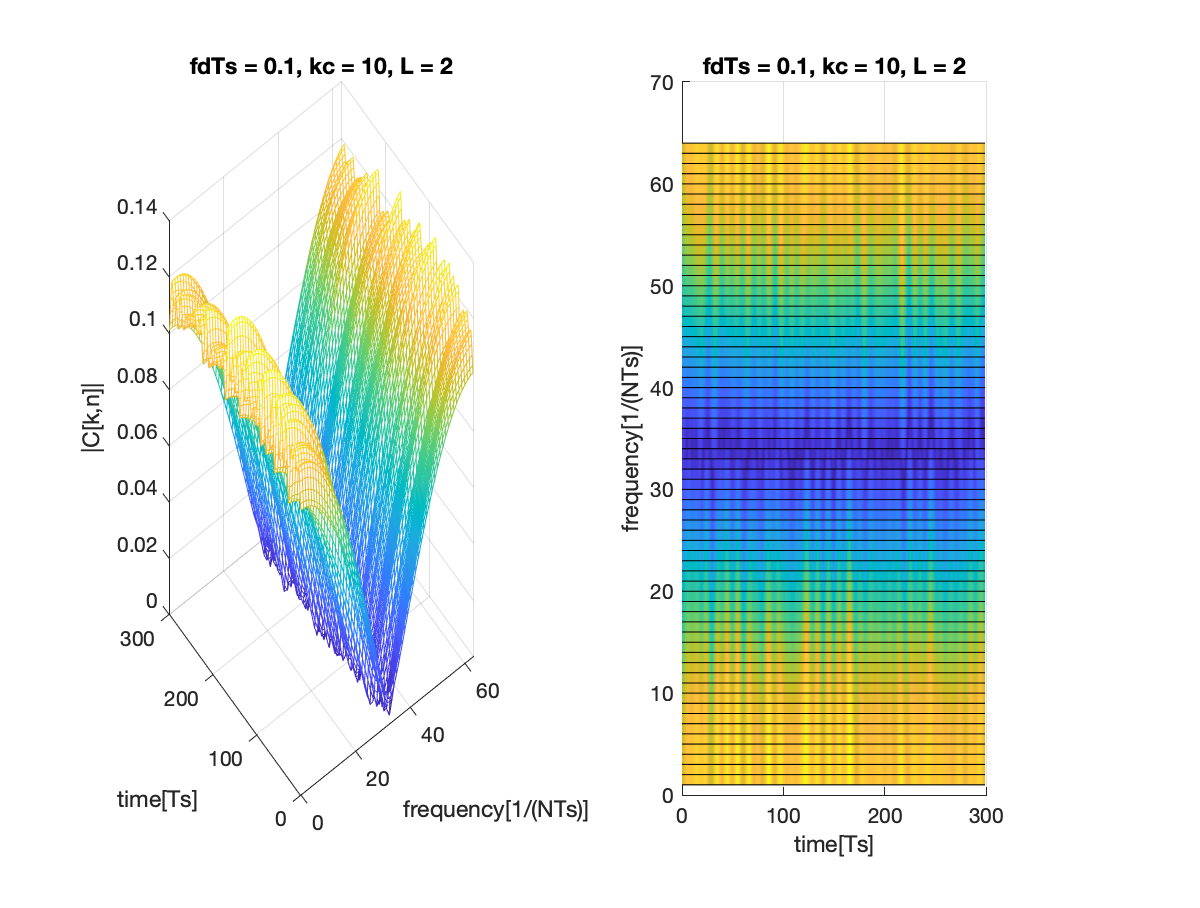
\includegraphics[width=\linewidth]{Task2/01_10_2.eps}
        \caption{$f_{D}T_{s}=0.1$,$k_{c}=10$,$L=2$}
        \label{01_10_2}
    \end{figure}
    \begin{figure}[H]
        \centering
        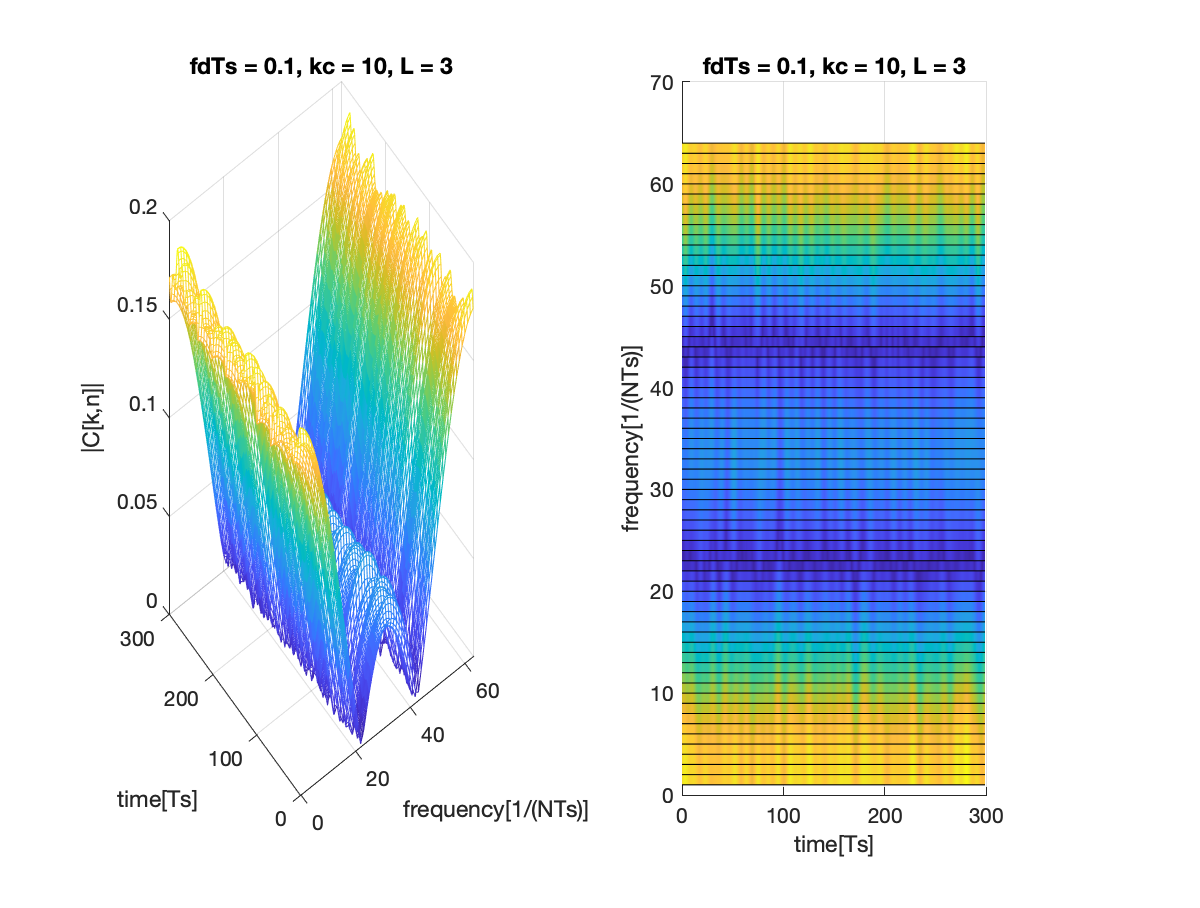
\includegraphics[width=\linewidth]{Task2/01_10_3.eps}
        \caption{$f_{D}T_{s}=0.1$,$k_{c}=10$,$L=3$}
        \label{01_10_3}
    \end{figure}
    \begin{figure}[H]
        \centering
        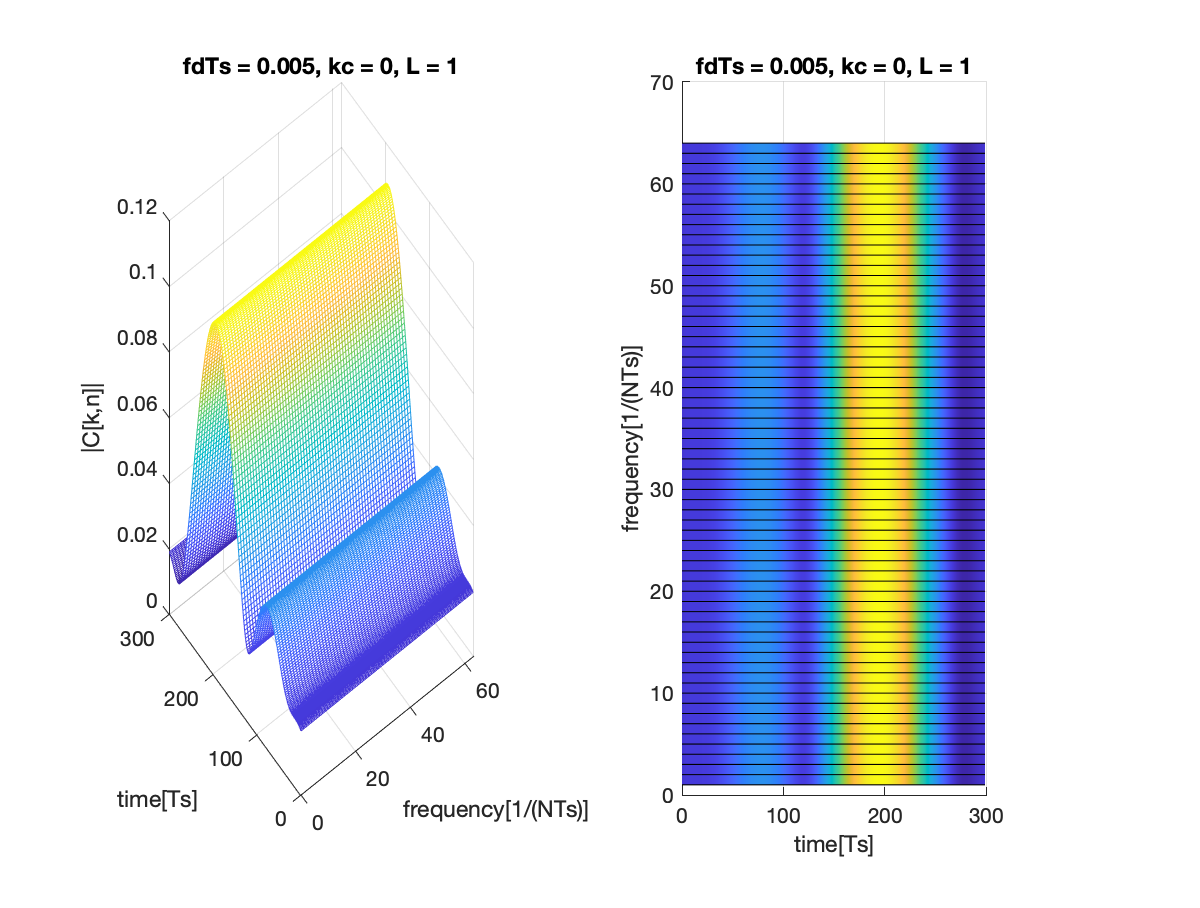
\includegraphics[width=\linewidth]{Task2/0005_0_1.eps}
        \caption{$f_{D}T_{s}=0.005$,$k_{c}=0$,$L=1$}
        \label{0005_0_1}
    \end{figure}
    \begin{figure}[H]
        \centering
        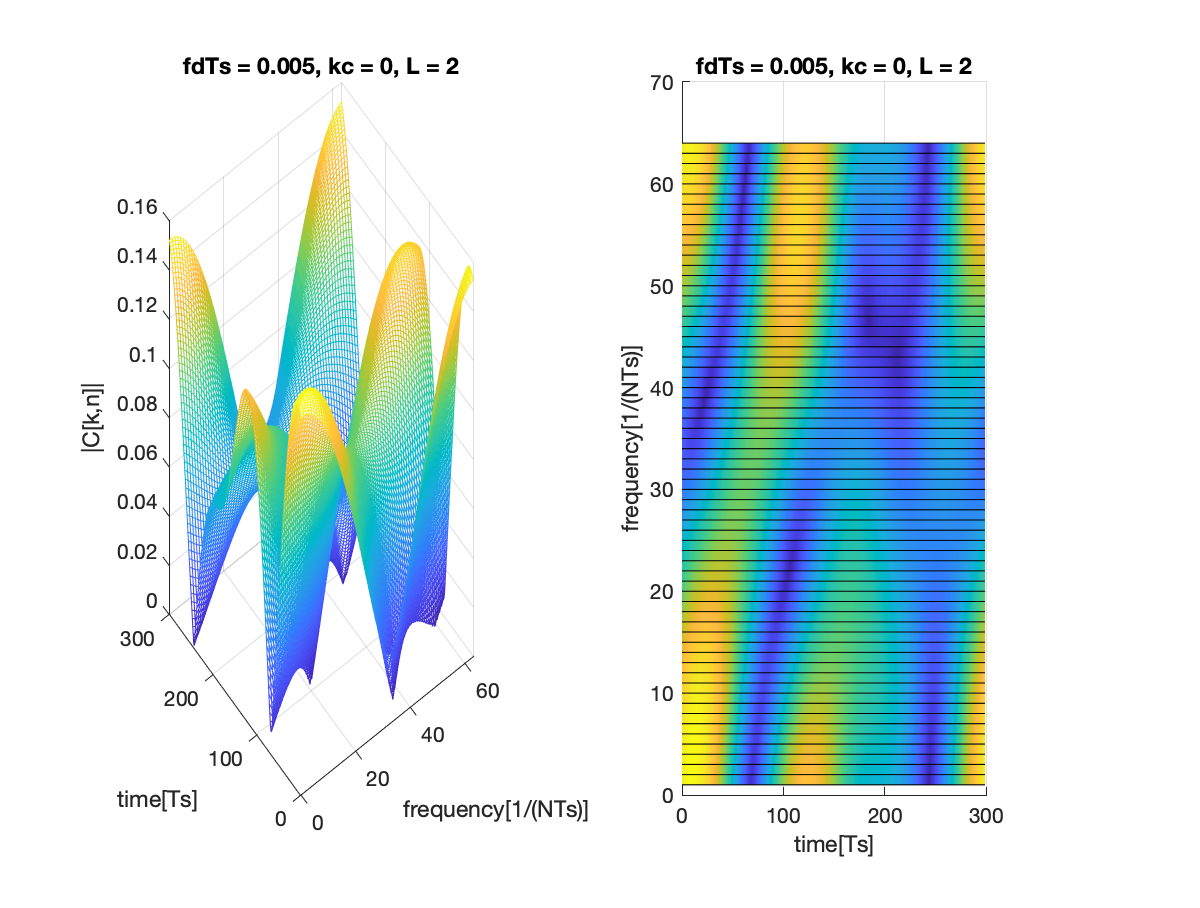
\includegraphics[width=\linewidth]{Task2/0005_0_2.eps}
        \caption{$f_{D}T_{s}=0.005$,$k_{c}=0$,$L=2$}
        \label{0005_0_2}
    \end{figure}
    \begin{figure}[H]
        \centering
        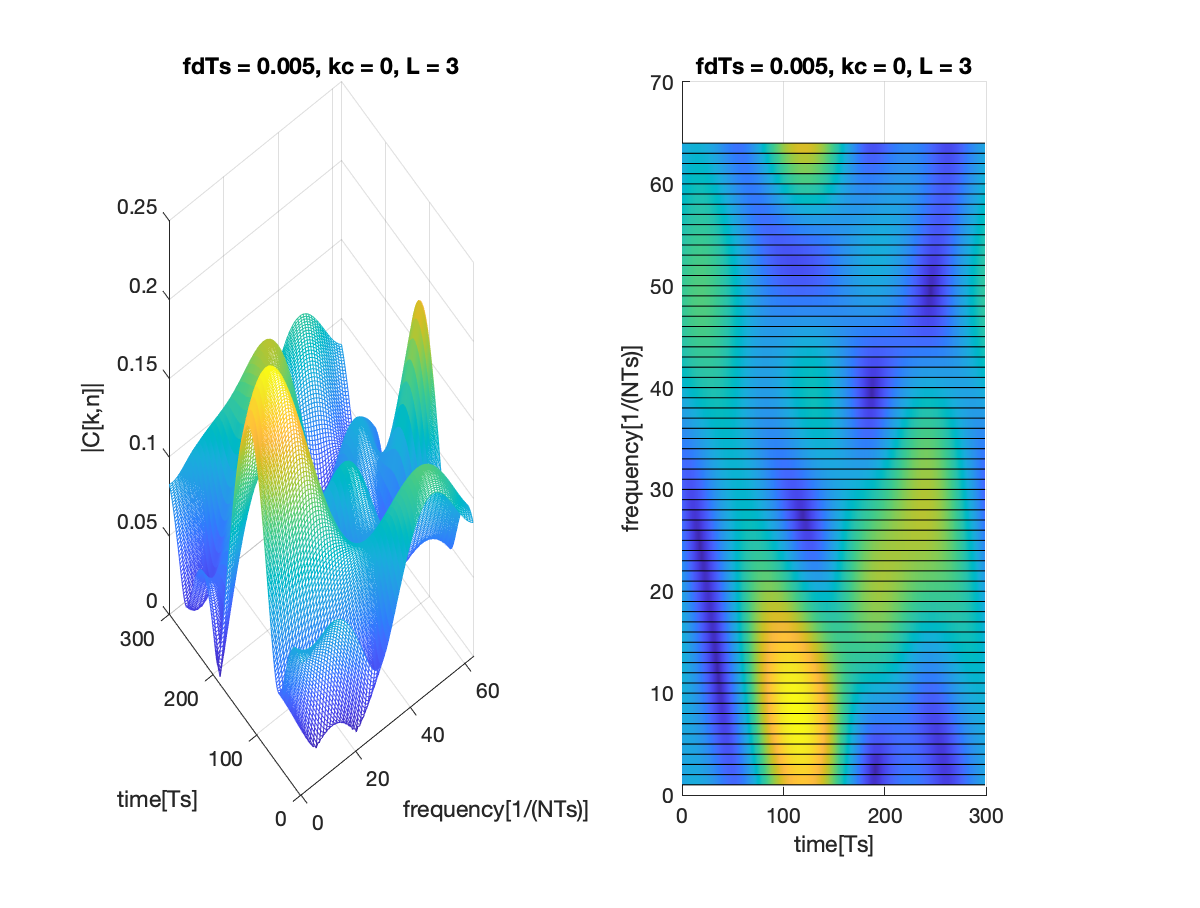
\includegraphics[width=\linewidth]{Task2/0005_0_3.eps}
        \caption{$f_{D}T_{s}=0.005$,$k_{c}=0$,$L=3$}
        \label{0005_0_3}
    \end{figure}
    \begin{figure}[H]
        \centering
        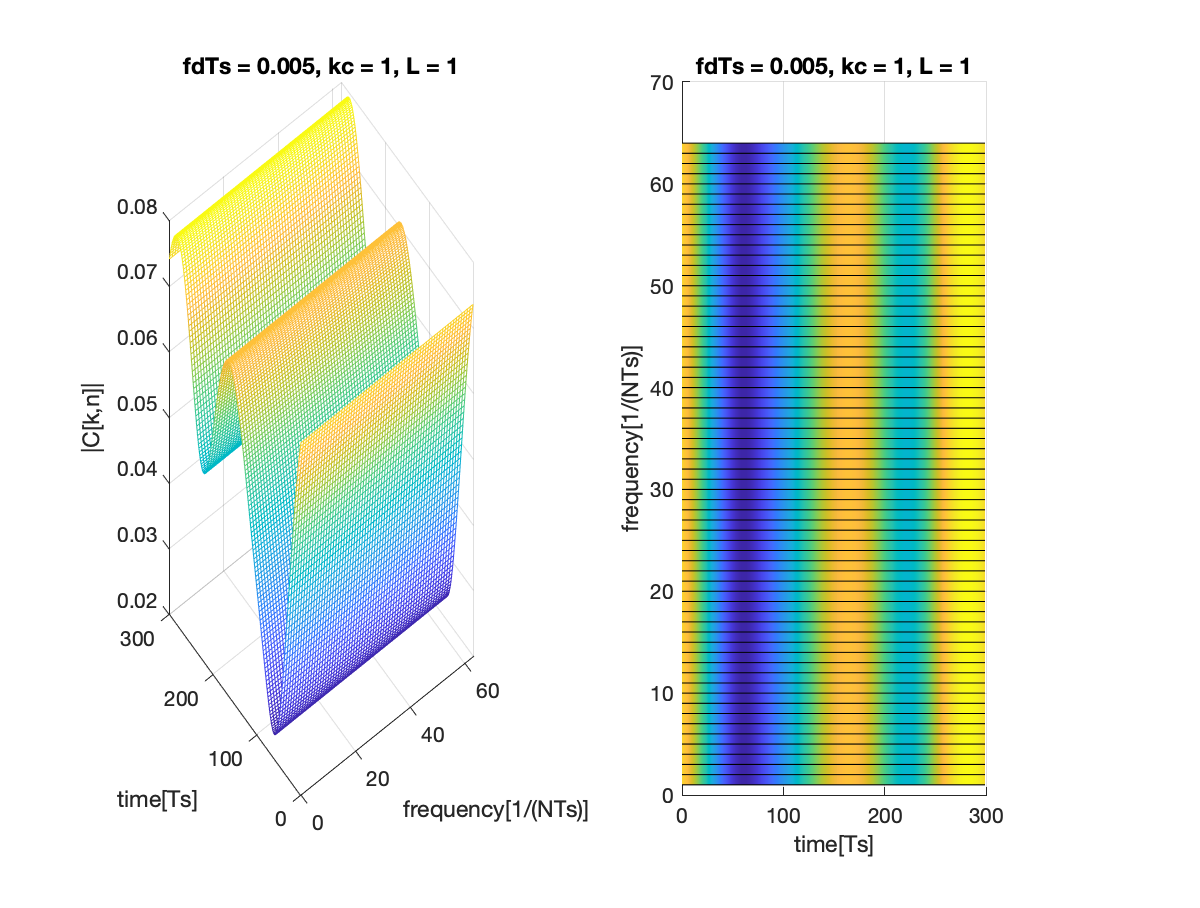
\includegraphics[width=\linewidth]{Task2/0005_1_1.eps}
        \caption{$f_{D}T_{s}=0.005$,$k_{c}=1$,$L=1$}
        \label{0005_1_1}
    \end{figure}
    \begin{figure}[H]
        \centering
        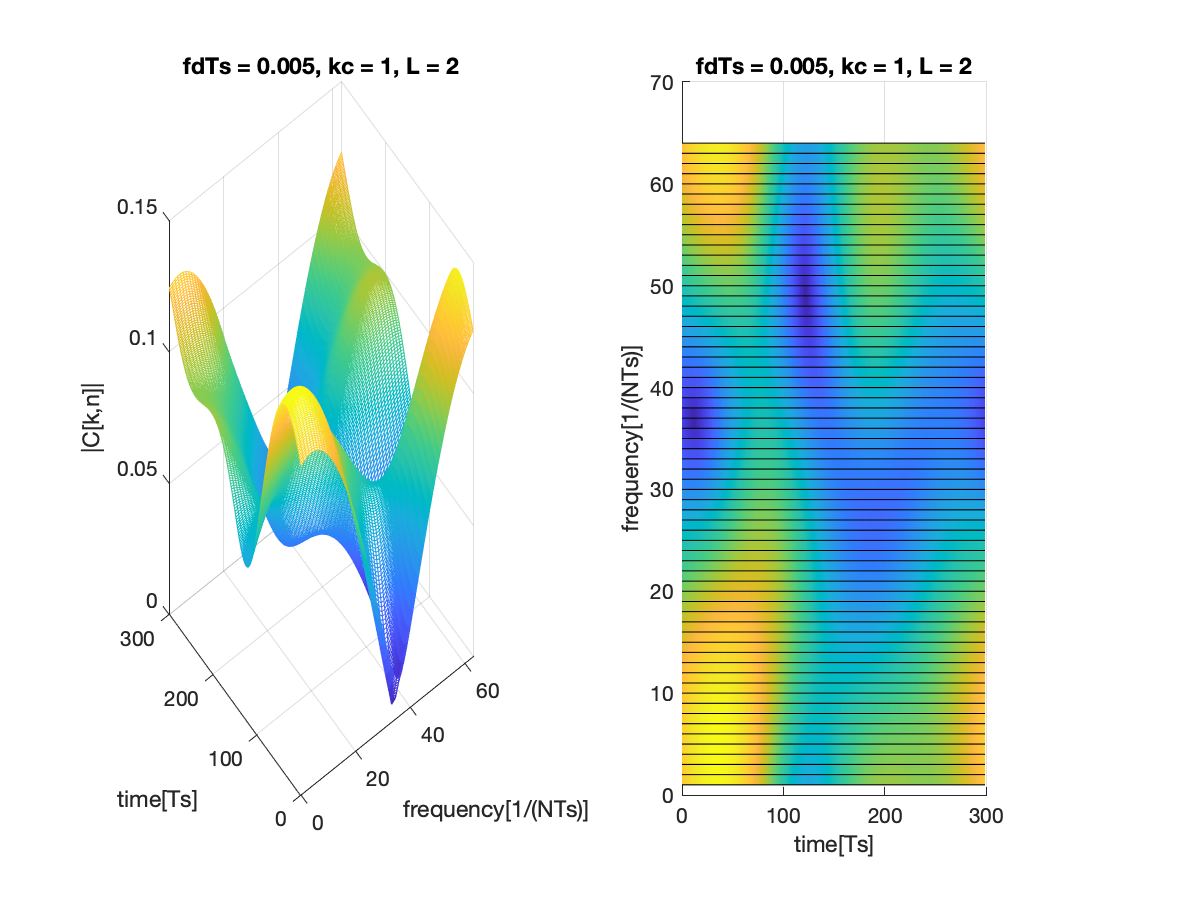
\includegraphics[width=\linewidth]{Task2/0005_1_2.eps}
        \caption{$f_{D}T_{s}=0.005$,$k_{c}=1$,$L=2$}
        \label{0005_1_2}
    \end{figure}
    \begin{figure}[H]
        \centering
        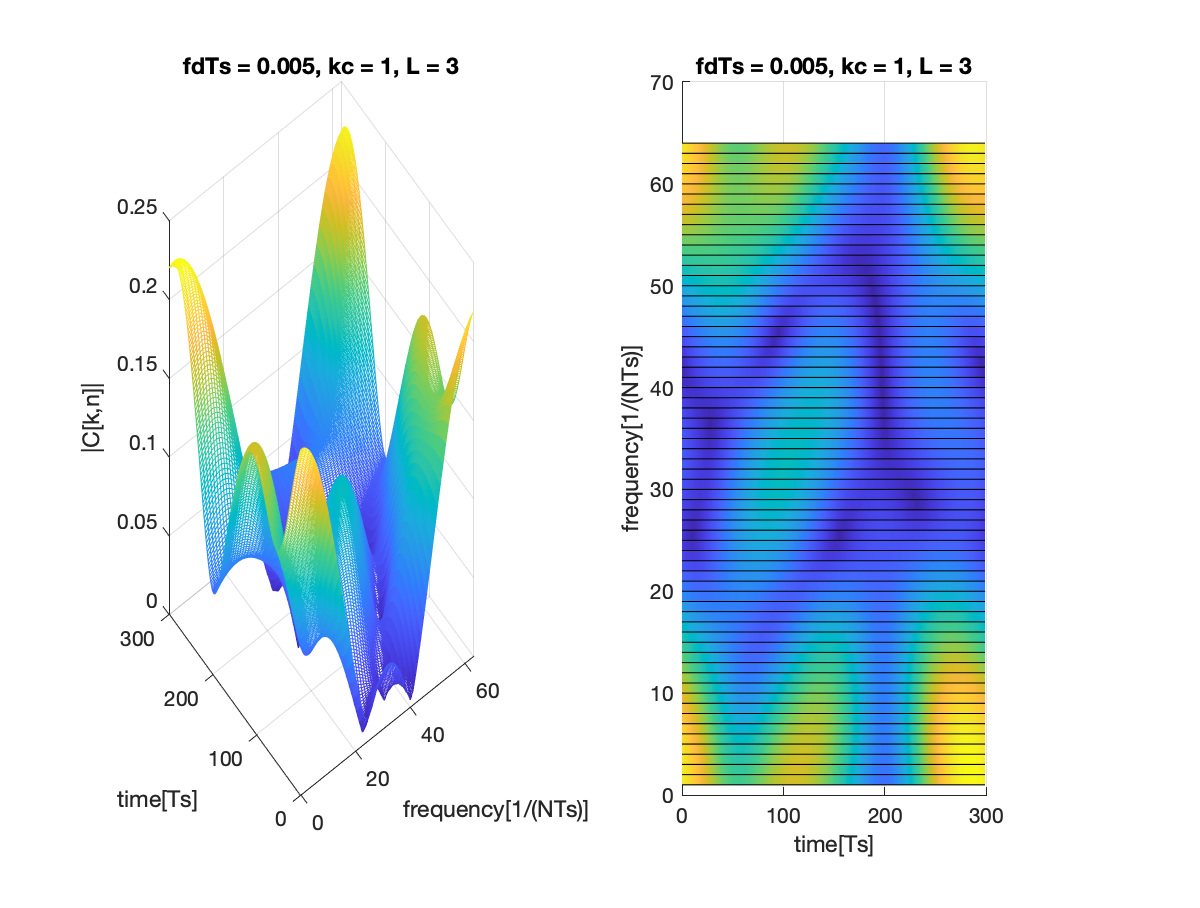
\includegraphics[width=\linewidth]{Task2/0005_1_3.eps}
        \caption{$f_{D}T_{s}=0.005$,$k_{c}=1$,$L=3$}
        \label{0005_1_3}
    \end{figure}
    \begin{figure}[H]
        \centering
        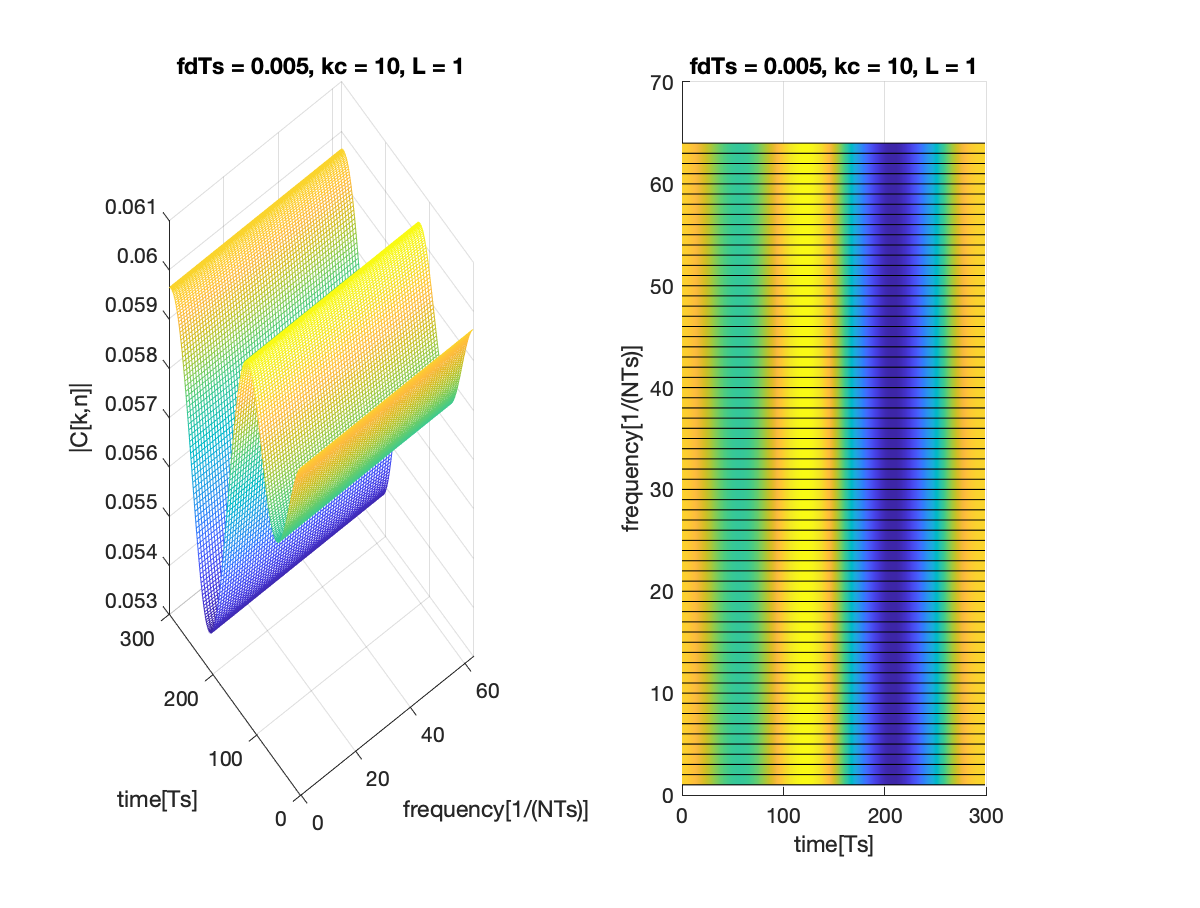
\includegraphics[width=\linewidth]{Task2/0005_10_1.eps}
        \caption{$f_{D}T_{s}=0.005$,$k_{c}=10$,$L=1$}
        \label{0005_10_1}
    \end{figure}
    \begin{figure}[H]
        \centering
        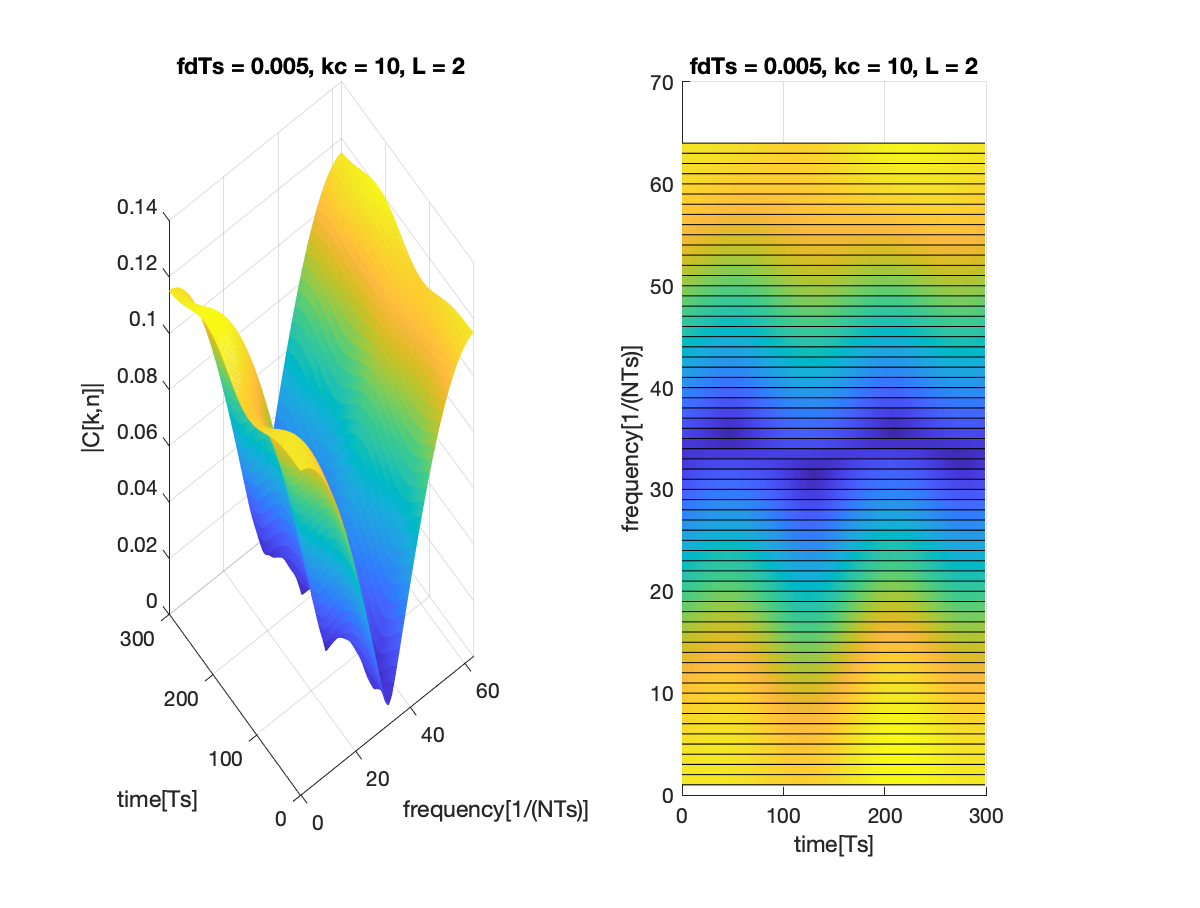
\includegraphics[width=\linewidth]{Task2/0005_10_2.eps}
        \caption{$f_{D}T_{s}=0.005$,$k_{c}=10$,$L=2$}
        \label{0005_10_2}
    \end{figure}
    \begin{figure}[H]
        \centering
        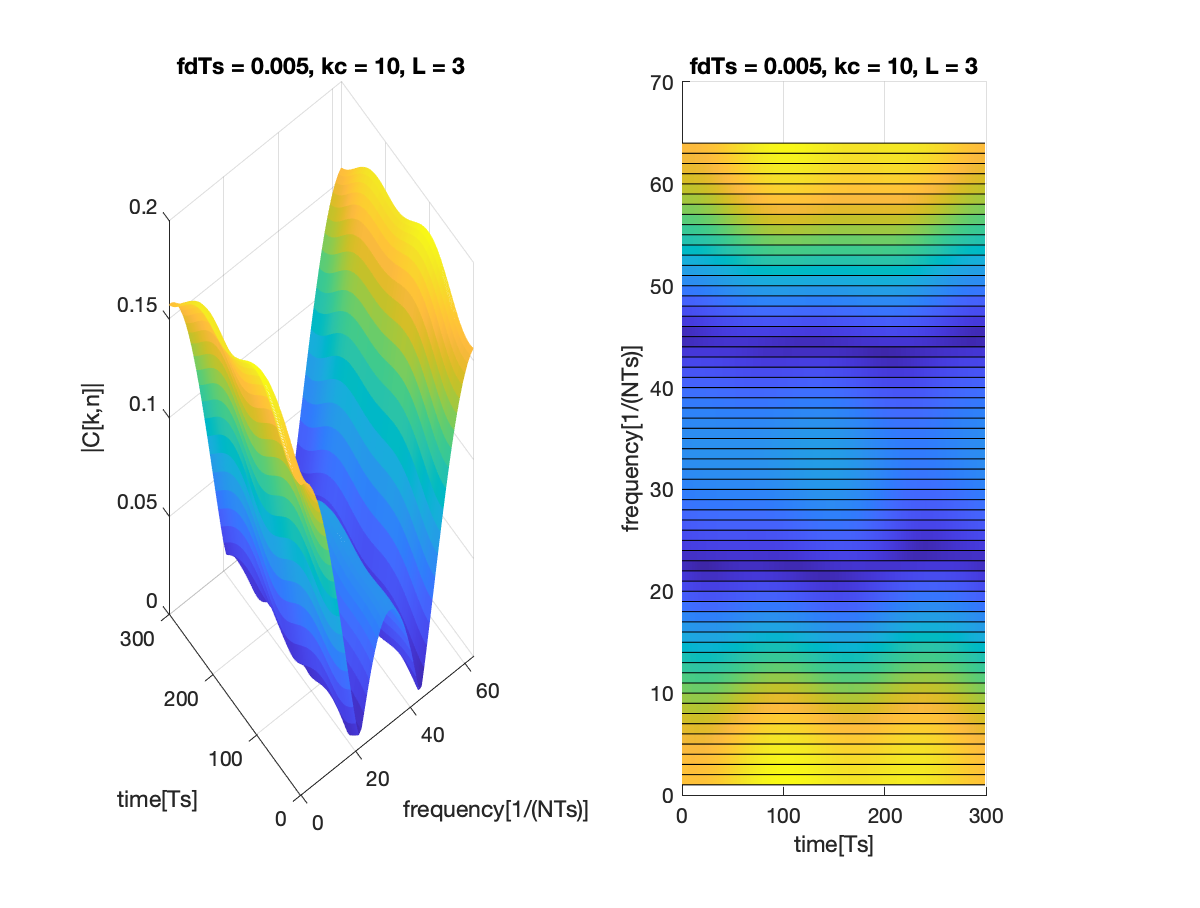
\includegraphics[width=\linewidth]{Task2/0005_10_3.eps}
        \caption{$f_{D}T_{s}=0.005$,$k_{c}=10$,$L=3$}
        \label{0005_10_3}
    \end{figure}
    \newpage
\section{}
    Here the MATLAB code written by the authors are given.
    

\lstset{language=Matlab,%
    %basicstyle=\color{red},
    breaklines=true,%
    morekeywords={matlab2tikz},
    keywordstyle=\color{blue},%
    morekeywords=[2]{1}, keywordstyle=[2]{\color{black}},
    identifierstyle=\color{black},%
    stringstyle=\color{mylilas},
    commentstyle=\color{mygreen},%
    showstringspaces=false,%without this there will be a symbol in the places where there is a space
    numbers=left,%
    numberstyle={\tiny \color{black}},% size of the numbers
    numbersep=9pt, % this defines how far the numbers are from the text
    emph=[1]{for,end,break},emphstyle=[1]\color{red}, %some words to emphasise
    %emph=[2]{word1,word2}, emphstyle=[2]{style},    
}


\lstinputlisting{MATLAB/project.m}
\lstinputlisting{MATLAB/filterMethod.m}
\lstinputlisting{MATLAB/spectrumMethod.m}
\lstinputlisting{MATLAB/padWithZeros.m}


\end{appendices}


\end{document}
